\documentclass[12pt]{article}
\usepackage{extsizes}
\usepackage{amsmath}
\usepackage{tikz}
\usepackage{graphicx}
\usepackage{subcaption}

\setlength{\oddsidemargin}{0in}
\setlength{\evensidemargin}{0in}
\setlength{\textheight}{9in}
\setlength{\textwidth}{6.5in}
\setlength{\topmargin}{-0.5in}
\setlength{\parskip}{1em}
\setlength{\parindent}{2em}

% Sample macros -- how you define new commands
% My own set of frequently-used macros have grown to many hundreds of lines.
% Here are some simple samples.

\newcommand{\Adv}{{\mathbf{Adv}}}          %example macro 
\newcommand{\getsr}{{\:\stackrel{{\scriptscriptstyle\hspace{0.2em}\$}}{\leftarrow}\:}}  % a more complex sample macro
\newcommand{\Func}[1]{{\mathrm{Fun}[{#1}]}}       % These macros take one
\newcommand{\Randd}[2]{{\mathrm{Rand}[{#1},{#2}]}} % and two arguments


%%%%%%%%%%%%%%%%%%%%%%%%%%%%%%%%%%%%%%%%%%%%%%%%%%%%%%%%%%%%%%%%%%%%%%%%%%%
\title{\bf Discrete II Final Project\\[2ex] 
       \rm\normalsize MATH 307 --- Spring 2019}
\date{\today}
\author{\bf Garrett Brenner}
\linespread{1.3}
\begin{document}
\maketitle

\pagebreak

%%%%%%%%%%%%%%%%%%%%%%%%%%%%%%%%%%%%%%%%%%%%%%%%%%%%%%%%
\section*{Abstract}

\begin{figure}[h]
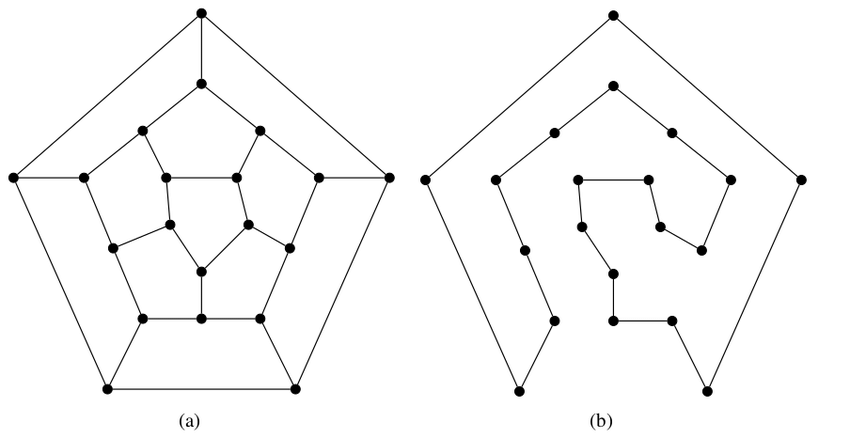
\includegraphics[scale=.5]{HamiltonCycle}
\centering
\end{figure}

For my Discrete II Final Project, I have elected to focus on a real-world
application of \textit{The Travelling Salesman Problem}. My goal is to use
a graphing algorithm to find the shortest path between each state in the US
and to model this with an animation. I use data collected from the Bureau 
of Transportation Statistics to model flight connections between each of 
these states (excluding Hawaii and Alaska, as they are not located within the
same continent).

%%%%%%%%%%%%%%%%%%%%%%%%%%%%%%%%%%%%%%%%%%%%%%%%%%%%%%%%
\section*{Mathematical Theory} 

The Travelling Salesman Problem could be briefly summarized as such: given
a set of cities and the distances between them (if such a path exists),
find the shortest possible route that visits every city in the set exactly
once and then returns to the starting city.

In Graph Theory, a Hamiltonian Cycle exists on a graph \(G = (V,E)\) if 
there exists a path between each vertex \(v \in V\) that only touches
each vertex once and returns to the starting vertex, in essence, creating
a cycle.

\pagebreak

If each city is considered a vertex and each route between them an edge,
it can be seen that the TSP resembles the problem of finding the shortest
possible Hamiltonian Cycle for \(G = (\)the set of cities $,$ the set of
paths between cities$)$.

This problem is NP-hard as well as NP-complete, essentially stating that
an algorithm's best case completion time is the same as its worst case and
furthermore that its worst case increases as much as exponentially with
each additional city. This factor comes into play later on.

%%%%%%%%%%%%%%%%%%%%%%%%%%%%%%%%%%%%%%%%%%%%%%%%%%%%%%%%
\section*{Procedure} 
I began by searching for a list of flight information that I could use to
build a graph. I found a .csv exportable list of regularly scheduled flights
on the Bureau of Transportation Statistics website. The unaltered file had 4123
rows as well as several additional columns which I deleted until all that
remained was "Row Number", "Origin", and "Destination". 

\begin{figure}[h]
       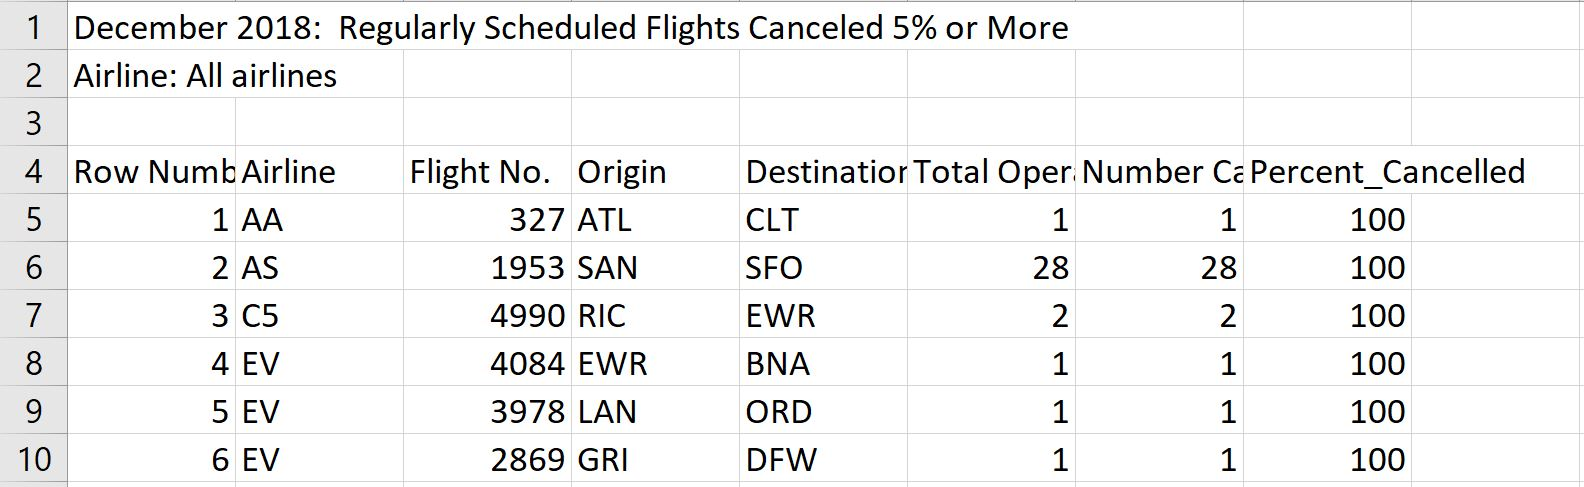
\includegraphics{originaldata}
       \centering
\end{figure}

To be a true Travelling Salesman problem designed to visit each state only
once, I only needed one airport from each state to represent visiting the
state as a whole. To accomplish this, I went through the list of states in
the US, excluding Hawaii and Alaska and selected what I assumed to be the
most popular (sharing the most edges with other airports) airport for each
one and adding their airport codes to a list. The reason for choosing the 
most popular airports was to aid increasing the probability of a multitude
of Hamiltonian Cycles between them.

\pagebreak
\begin{center}
       \textit{Set of Airports}: \{MGM, ANC,
       PHX,
       LIT,
       SMF,
       DEN,
       BDL,
       ILG,
       MCO,
       ATL,
       HNL,
       BOI,
       ORD,
       IND,
       DSN,
       MCI,
       SDF,
       MSY,
       AUG,
       BWI,
       BOS,
       DTW,
       MSP,
       JAN,
       STL,
       BIL,
       LNK,
       LAS,
       MHT,
       EWR,
       ABQ,
       JFK,
       CLT,
       BIS,
       CMH,
       OKC,
       PDX,
       PHL,
       PVD,
       CHS,
       PIR,
       BNA,
       DFW,
       SLC,
       MPV,
       RIC,
       SEA,
       CRW,
       MSN,
       CYS\} 
\end{center}

At this point, not having a desire to manually edit a 4123 row long Excel
sheet, I knew I required the help of someone more experienced with data science. I tried applying
what I knew of the pandas an numpy libraries in Python to the data and 
Googling my way through, but to no avail. Thankfully, Data Science and
Economics double major Mackenzie Schaich was
willing to give up a few minutes of her time to help me. All work was done
in Jupyter Lab through Anaconda.

The first thing we needed to do was alphebatize the "Origin" column to
make the spreadsheet more readable and make it easier to identify errors.

\begin{figure}[h]
       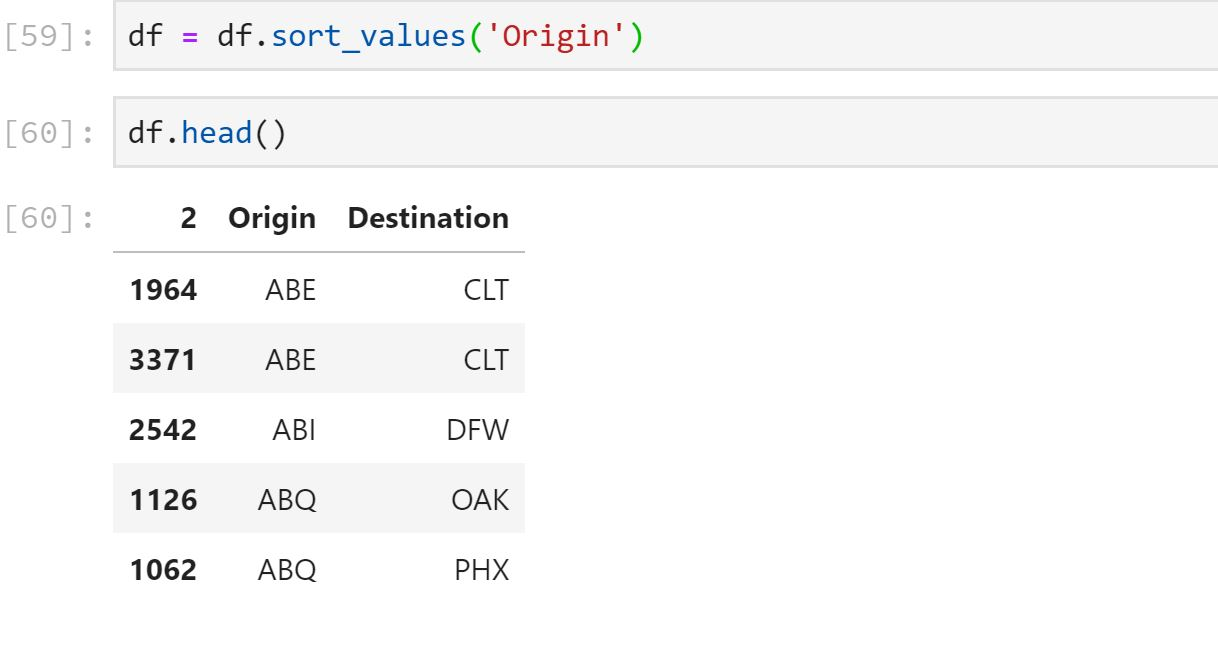
\includegraphics{alphabetize}
       \centering
\end{figure}

\pagebreak

Following this, all we had to do was remove all airports that were not in my
list of one airport per state which was a .txt file with each airport
delimited by a new line.

\begin{figure}[h]
       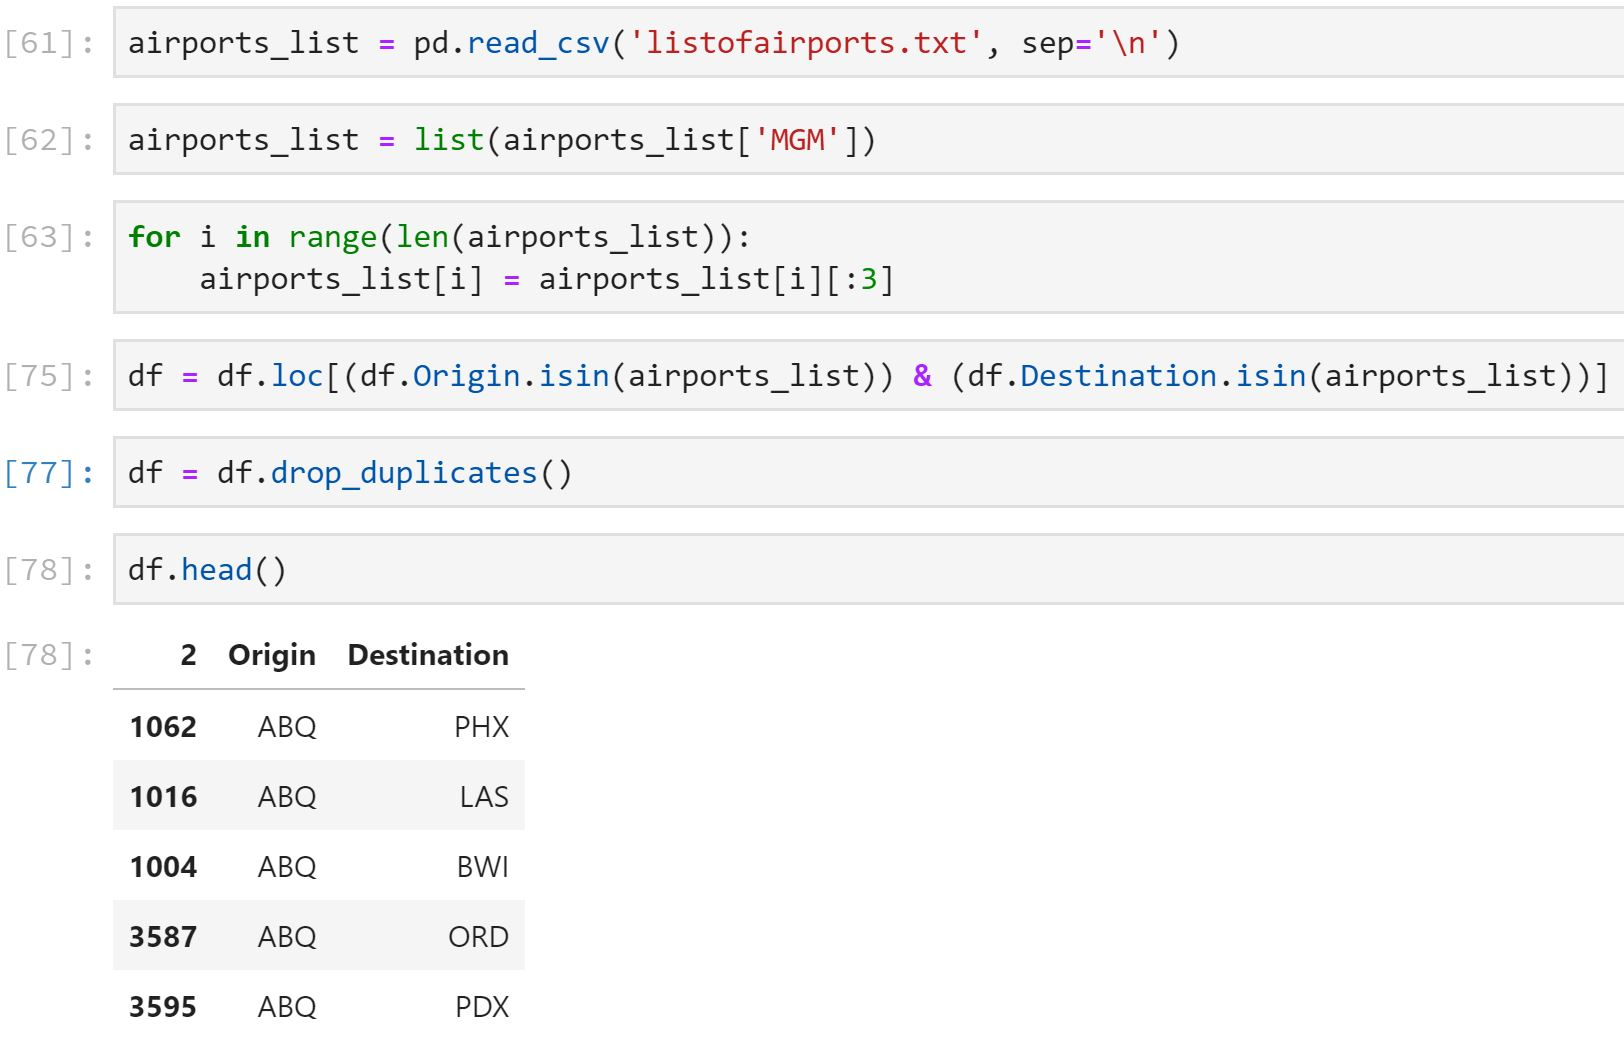
\includegraphics{dropdups}
       \centering
\end{figure}

Now that I had the data split into alphebatized chunks where
I could easily observe all destination airports from each origin airport,
I added a third column titled "Distance". Finally, I manually computed 
each distance using airmilescalculator.com and entered them into Excel. 
Next it was time to convert the .csv to .txt and open it up in Python.

At this point I was also considering how I was going to be graphing these
airports, hopefully in a way that loosely resembled their location on 
a map of the United States. In retrospect, it would have been a better idea
to just get the longitudinal and latitudinal coordinates for each of them,
but at the time I hadn't thought of that. For each airport in my list of
included airports, I manually looked up and wrote down a working address
and then did a bulk entry into mapcustomizer.com to view them all on a 
map of the US. After that, I was planning on using Photoshop to find the
pixel distance between the center of the model and each individual airport
in order to hopefully provide a basis for graphical representation,
but that plan didn't pan out.

I spent several days trying to install the iGraph library for Python to
help with the visualization, but I was never able to do it successfully.
Here, I feel I must interject
my personal distaste for that library and its monster of an installment 
process. Even now, it attempts to lure me with its beautiful visualizations,
but I shall not give in for I know it is unachievable. 

After that flopped, I was forced to do the entire project with no visualization
which was unfortunate, but did make it easier to code. I found an applicable
algorithm on geeksforgeeks.org written in C++ that solved the minimum Hamiltonian
cycle of a graph given an adjacency matrix and a source vertex and then returned
the total weight of that path. It was only a matter of translating that 
C++ into Python and making a few tweaks here and there before I was able to get
it working on a sample graph provided by the website. At this point, I took
the liberty of also implementing the ability to view the entire Hamiltonian path,
not just the total weight. In layman's terms, whereas before the screen might
show 8000 miles to represent the minimum distance visiting each state and returning,
it now would also show the sequence of airports one would take to achieve such a path.

\pagebreak

\begin{figure}[h]
       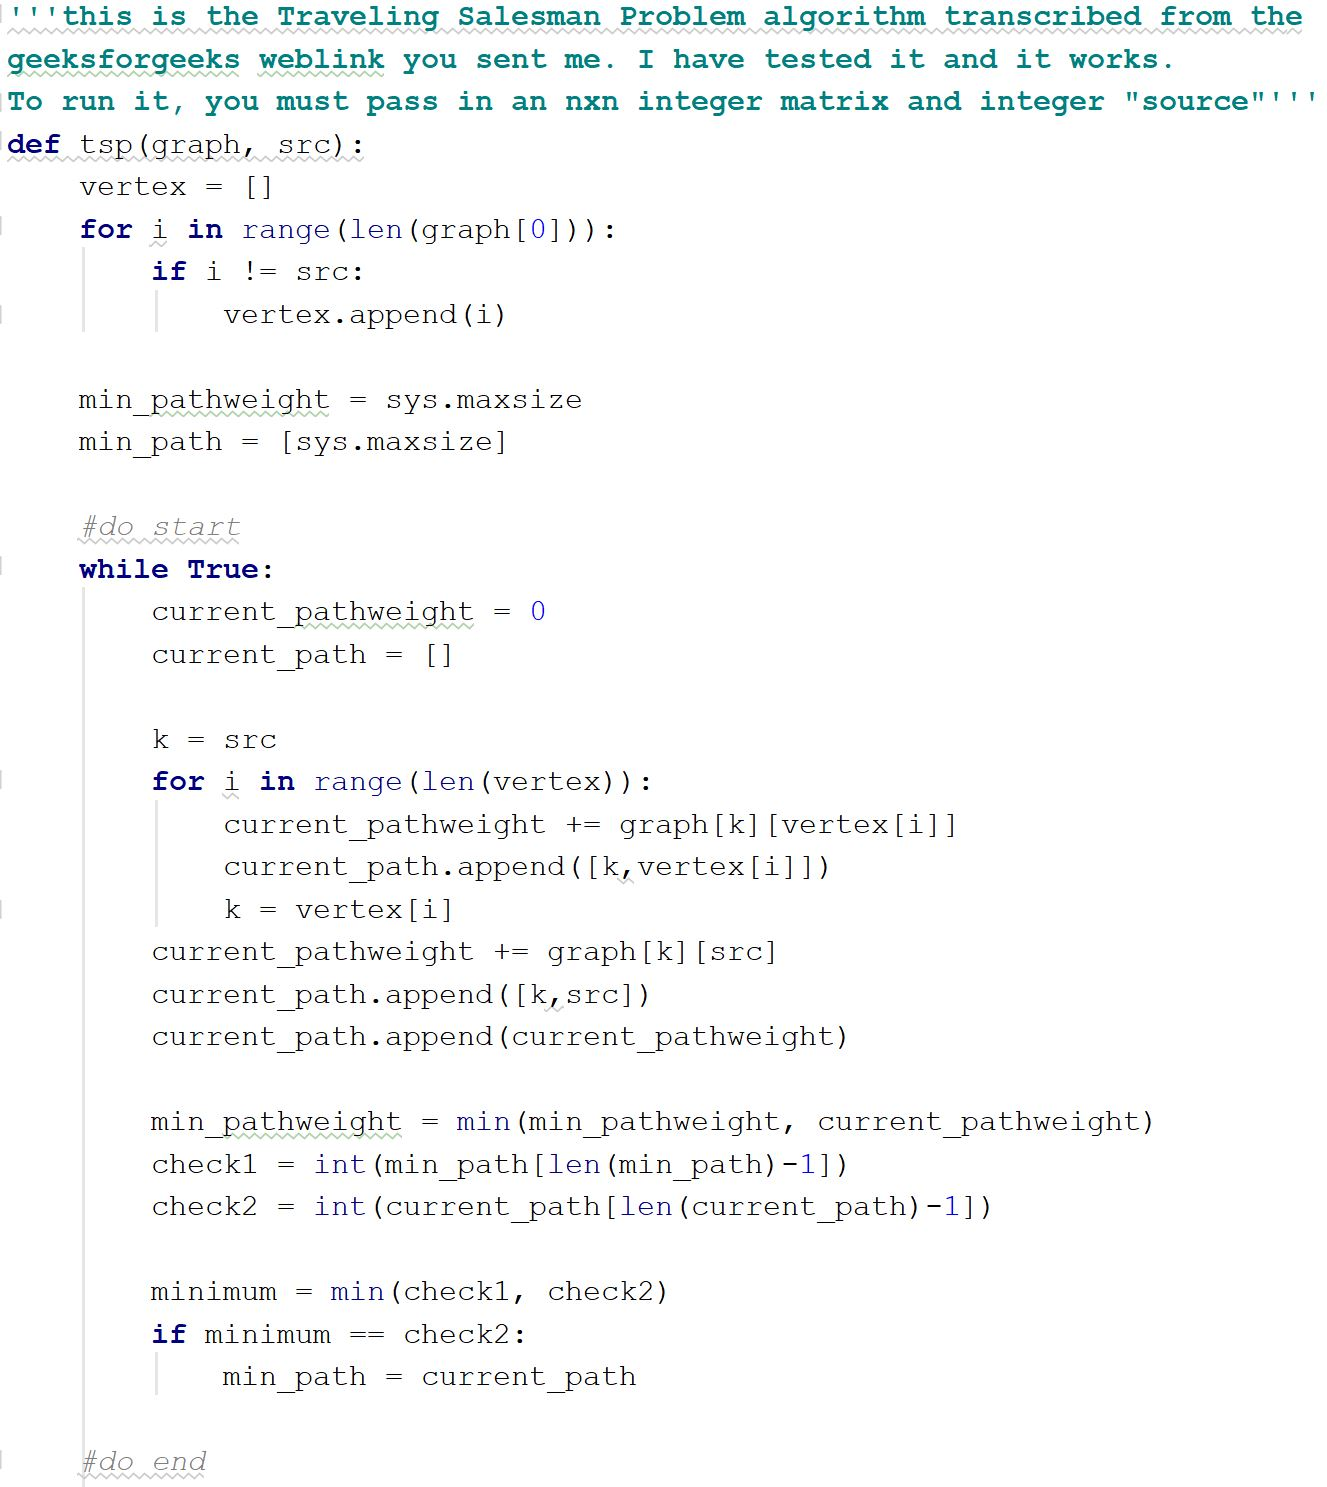
\includegraphics[scale=.85]{code1}
       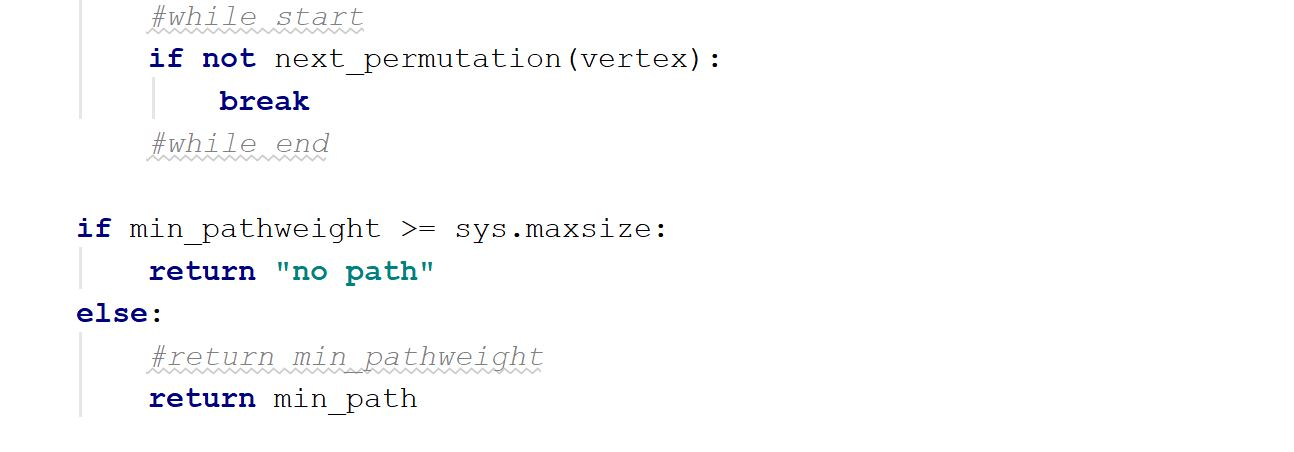
\includegraphics[scale=.85]{code2}
       \centering
\end{figure}

Here's where the time complexity comes into play. As was noted by the author
of the geeksforgeeks article, the time complexity of the algorithm was \(O(n!)\)
where $n$ is the number of cities. For example, calculating the minimum cycle with
four cities takes four times as long as calculating it with three cities because
\[(4)! = 4 \cdot (3)! = 4 \cdot 3 \cdot (2)! = 4 \cdot 3 \cdot 2 \cdot 1\]
My data contained 42 unique airports for the algorithm to work with. 
\[(42)! \approx 1400000000000000000000000000000000000000000000000000\] So you
can try to comprehend how long that might take for a computer to solve. This
meant I would not be able to solve the original problem I had set out to solve,
not because I couldn't find a solution, but simply because it would just take
too long. However, solving smaller problems like with 10 airports instead of 42
is easy for my computer. Below demonstrates an adjacency matrix (e.g. the distance
going from airport$_0$ to airport$_2$ is represented by M$_{0,2}$) for 10 airports: 
DFW, ABQ, PHX, LAS, BWI, ORD, PDX, DEN, MCI, MCO, ATL. If an element in the matrix
is $\infty$ that means there is no path between those two airports (at least
in that direction, as M$_{0,2}$ may not exist but M$_{2,0}$ can).

\[
\quad
\begin{bmatrix}
       0 & 569 & 868 & 1055 & 1217 & 802 & 1616 & 641 & 460 & 985 \\
       569 & 0 & 328 & 486 & 1670 & 1118 & 1111 & 349 & 718 & 1553 \\
       868 & 328 & 0 & \infty & \infty & 1440 & 1009 & 602 & 1044 & \infty \\
       1055 & 486 & 255 & 0 & \infty & \infty & \infty & \infty & \infty & \infty \\
       1217 & 1670 & 1999 & \infty & 0 & \infty & \infty & \infty & \infty & 787 \\
       802 & 1118 & 1440 & \infty & \infty & 0 & \infty & \infty & 403 & 1005 \\
       1616 & \infty & 1009 & \infty & \infty & \infty & 0 & \infty & \infty & \infty \\
       641 & 349 & 602 & 628 & 1491 & \infty & \infty & 0 & 533 & \infty \\
       460 & \infty & 1044 & \infty & \infty & 403 & \infty & \infty & 0 & \infty \\
       985 & 1553 & \infty & \infty & 787 & \infty & \infty & \infty & \infty & 0 \\
\end{bmatrix}
\quad
\]

Professor Kumar connected me with the College of
Charleston's high performance computing so I altered my code to begin at a 
4x4 adjacency matrix and work its way up to a 42 x 42 adjacency matrix and sent 
it over just to see how far it could get. I also changed the source vertex to
be the Dallas Fort Worth airport because it has the most connections.

%%%%%%%%%%%%%%%%%%%%%%%%%%%%%%%%%%%%%%%%%%%%%%%%%%%%%%%%
\section*{Results and Conclusion} 

The highest result I was able to get on my computer within a reasonable amount
of time was using an 11x11 matrix. The returned path and path weight were as
follows:

\begin{center}
[['DFW', 'LAS'], ['LAS', 'ABQ'], ['ABQ', 'PDX'], ['PDX', 'PHX'],
 ['PHX', 'DEN'], ['DEN', 'MCI'], ['MCI', 'ORD'], ['ORD', 'ATL'], 
 ['ATL', 'BWI'], ['BWI', 'MCO'], ['MCO', 'DFW'],] 8154 miles is the minimum distance
\end{center}

The highest result I was able to get on the high performance computer within
a reasonable amount of time was using a blankxblank matrix. The returned path and
weight were as follows:

\begin{center}
       [] m miles is the minimum distance
       \end{center}

\section*{References}

Singh, N. (2017, November 11). Traveling Salesman Problem (TSP) Implementation. Retrieved from https://www.geeksforgeeks.org/traveling-salesman-problem-tsp-implementation/

\end{document}